% =====================================================================
% PHYS 400 -- A0 research poster (portrait), academic/formal design
% Automated Construction of Multi-Element MEAM Interatomic Potentials
%
% Design language: journal page, not billboard. Palatino text + math
% (mathpazo), white ground, hairline rules, numbered small-caps
% sections, formal figure/table captions. The METU darkred appears
% only as an accent: section numbers, rules, key results.
%
% Build with ./compile.sh. Figures are the committed PNGs copied from
% reports/finalPresentation/figures; regenerate them there.
% =====================================================================
\documentclass[a0,portrait]{a0poster}

\usepackage[utf8]{inputenc}
\usepackage[T1]{fontenc}
\usepackage[osf,sc]{mathpazo}          % Palatino text + matching math
\linespread{1.0}
\usepackage{amsmath}
\usepackage{graphicx}
\usepackage{booktabs}
\usepackage{multicol}
\usepackage[letterspace=120]{microtype} % letterspacing for the kicker
\usepackage{tikz}
\usetikzlibrary{arrows.meta, positioning}
\usepackage{tcolorbox}                  % only for the thin-rule result blocks
\tcbuselibrary{skins}
\usepackage{qrcode}
\usepackage{needspace}
\usepackage[margin=3cm]{geometry}
\pagestyle{empty}
\parindent=0pt
\parskip=0.5em

% --- palette: ink on paper, METU red carried through -------------------
\definecolor{ink}{HTML}{1C1A19}
\definecolor{accent}{HTML}{CC0000}      % METU red, exact match to the logo
\colorlet{hairline}{accent!35}          % red-tinted hairlines
\color{ink}

% --- numbered small-caps section heading with hairline ----------------
\newcounter{sec}
\newcommand{\sect}[1]{%
  \stepcounter{sec}%
  \Needspace*{8\baselineskip}%
  \vspace{0.9em}%
  {\LARGE\raggedright\hyphenpenalty=10000\color{accent}
   {\bfseries\thesec.}\hspace{0.55em}{\scshape #1}\par}%
  \vspace{0.28em}{\color{hairline}\hrule height 0.6pt}\vspace{0.55em}}

% --- formal figure / table captions ------------------------------------
\newcounter{fig}
\newcommand{\figcap}[1]{\stepcounter{fig}\par\vspace{0.3em}%
  {\small{\color{accent}\bfseries Figure~\thefig.} \ #1\par}}
\newcounter{tab}
\newcommand{\tabcap}[1]{\stepcounter{tab}\par\vspace{0.3em}%
  {\small{\color{accent}\bfseries Table~\thetab.} \ #1\par}}

% --- key-result block: accent rule on the left, light METU-red ground --
\newtcolorbox{keyresult}{enhanced, frame hidden, colback=accent!5,
  borderline west={3pt}{0pt}{accent}, sharp corners,
  left=6mm, right=4mm, top=2mm, bottom=2mm,
  before skip=0.8em, after skip=0.8em, fontupper=\normalsize}

\begin{document}

% =====================================================================
% Title block
% =====================================================================
\begin{tcolorbox}[enhanced, frame hidden, colback=accent, sharp corners,
  left=0mm, right=0mm, top=3mm, bottom=3mm, boxsep=0mm]
  \centering
  {\large\color{white}\textls{PHYS 400 SENIOR PROJECT \, $\cdot$ \,
    DEPARTMENT OF PHYSICS \, $\cdot$ \,
    MIDDLE EAST TECHNICAL UNIVERSITY}\par}
\end{tcolorbox}

\vspace{0.4em}
\begin{minipage}[c]{0.10\linewidth}
  
\includegraphics[width=0.78\linewidth]{metu.png}
\end{minipage}\hfill
\begin{minipage}[c]{0.78\linewidth}
  \centering
  {\VeryHuge\bfseries\color{accent} Automated Construction of Multi-Element\par}
  \vspace{0.12em}
  {\VeryHuge\bfseries\color{accent} MEAM Interatomic Potentials\par}
  \vspace{0.5em}
  {\LARGE\itshape A DFT-informed neural-network optimization framework\par}
  \vspace{0.85em}
  {\Large Can Durmaz\quad$\cdot$\quad
   Advisor: Prof.\ Dr.\ Hande Toffoli\par}
\end{minipage}\hfill
\begin{minipage}[c]{0.082\linewidth}
  \centering
  {\color{accent}\qrcode[height=\linewidth]{https://github.com/canndurmaz/PHYS400}}\\[1.5mm]
  {\scriptsize\color{accent} code \& data}
\end{minipage}

\vspace{0.7em}
{\color{accent}\hrule height 1.6pt}\vspace{2.5pt}{\color{accent}\hrule height 0.5pt}
\vspace{0.8em}

% =====================================================================
% Figure 1: the pipeline, full width, formal styling
% =====================================================================
\begin{center}
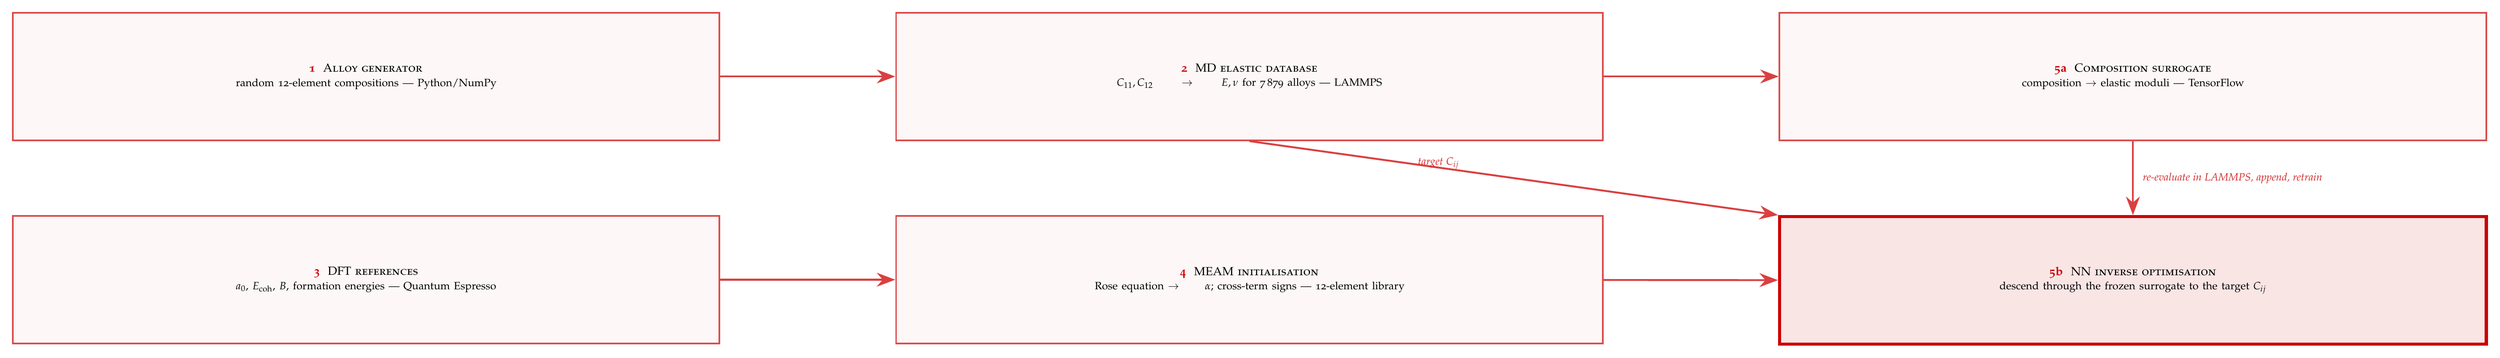
\begin{tikzpicture}[
    stage/.style={rectangle, draw=accent!70, line width=1.4pt, fill=accent!3,
      text width=200mm, minimum height=38mm, align=center, font=\normalsize,
      inner sep=5mm},
    emphstage/.style={stage, draw=accent, line width=2.6pt, fill=accent!10},
    snum/.style={font=\normalsize\bfseries, text=accent},
    arr/.style={-{Stealth[length=5.5mm]}, line width=1.6pt, accent!75},
    lab/.style={font=\small\itshape, text=accent!85},
  ]
  % top track: configuration data
  \node[stage] (gen) {{\color{accent}\bfseries 1}\ \ {\scshape Alloy generator}\\
    {\small random 12-element compositions --- Python/NumPy}};
  \node[stage, right=52mm of gen] (md) {{\color{accent}\bfseries 2}\ \ {\scshape MD elastic database}\\
    {\small $C_{11},C_{12}\to E,\nu$ for 7\,879 alloys --- LAMMPS}};
  \node[stage, right=52mm of md] (nn5a) {{\color{accent}\bfseries 5a}\ \ {\scshape Composition surrogate}\\
    {\small composition $\to$ elastic moduli --- TensorFlow}};
  % bottom track: the potential
  \node[stage, below=22mm of gen] (dft) {{\color{accent}\bfseries 3}\ \ {\scshape DFT references}\\
    {\small $a_0$, $E_{\mathrm{coh}}$, $B$, formation energies --- Quantum Espresso}};
  \node[stage, below=22mm of md] (init) {{\color{accent}\bfseries 4}\ \ {\scshape MEAM initialisation}\\
    {\small Rose equation $\to\alpha$; cross-term signs --- 12-element library}};
  \node[emphstage, below=22mm of nn5a] (nn5b) {{\color{accent}\bfseries 5b}\ \ {\scshape NN inverse optimisation}\\
    {\small descend through the frozen surrogate to the target $C_{ij}$}};
  % flow
  \draw[arr] (gen) -- (md);
  \draw[arr] (md) -- (nn5a);
  \draw[arr] (dft) -- (init);
  \draw[arr] (init) -- (nn5b);
  \draw[arr] (md.south) -- node[lab, right=1.5mm, pos=0.3]{target $C_{ij}$}
    (nn5b.north west);
  \draw[arr] (nn5a.south) -- node[lab, right=1.5mm]{re-evaluate in LAMMPS, append, retrain}
    (nn5b.north);
\end{tikzpicture}
\end{center}
\begin{center}
\begin{minipage}{0.72\linewidth}
\figcap{The five-stage pipeline. The upper track assembles a
composition--property database; the lower track builds the potential
itself. Stage 5b closes the loop: optimized parameters are re-evaluated
in LAMMPS, appended to the training set, and the surrogate is retrained.}
\end{minipage}
\end{center}

\vspace{0.4em}

% =====================================================================
% Three-column body
% =====================================================================
\setlength{\columnsep}{20mm}
\setlength{\columnseprule}{0.5pt}
\renewcommand{\columnseprulecolor}{\color{hairline}}
\begin{multicols}{3}

% ------------------------------------------------------------ sec 1
\sect{Motivation \& objective}
The cubic stiffness constants $C_{11}$, $C_{12}$ --- and the derived
Young's modulus $E$ and Poisson's ratio $\nu$ --- are the principal
design criteria for structural alloys, yet measuring them is slow and
expensive. Classical molecular dynamics recovers the same properties at
negligible cost, \emph{provided} an accurate interatomic potential is
available. For metals the standard semi-empirical form is the Modified
Embedded Atom Method (MEAM) [1,\,2], whose parameters are traditionally
fitted by hand --- expert work that does not scale to many-element
alloys.

\begin{keyresult}
\textbf{Objective.} Construct MEAM potentials automatically for an
arbitrary set of elements, with no manual parameter fitting and no
experimental input.
\end{keyresult}

% ------------------------------------------------------------ sec 2
\sect{Random alloy generation}
Compositions are drawn uniformly on the 12-element simplex
(Al, Co, Cr, Cu, Fe, Mg, Mn, Mo, Ni, Si, Ti, Zn), weighted toward
aluminium to oversample the commercially dominant region. Of
${\sim}7\,900$ generated configurations, \textbf{7\,815 are retained}
by the physicality filter
($E>0$, $0<\nu<0.48$, $C_{11}>C_{12}$).

\begin{center}\begin{minipage}{\linewidth}\centering

\includegraphics[width=0.96\linewidth]{figures/element_frequency.png}
\figcap{Element occurrence over the retained corpus.}
\end{minipage}\end{center}

% ------------------------------------------------------------ sec 3
\sect{Molecular-dynamics elastic database}
Each configuration is realised as a ${\sim}4$\,nm cubic supercell in
LAMMPS [3] with the merged 12-element MEAM library. After anisotropic
energy minimisation, axial strains $\delta=10^{-3}$ along
$\pm x,\pm y,\pm z$ yield $C_{11}$ and $C_{12}$ by central differences;
$E$ and $\nu=C_{12}/(C_{11}+C_{12})$ follow analytically. Median
$E=103.6$\,GPa and median $\nu=0.326$ over the corpus.

\begin{center}\begin{minipage}{\linewidth}\centering
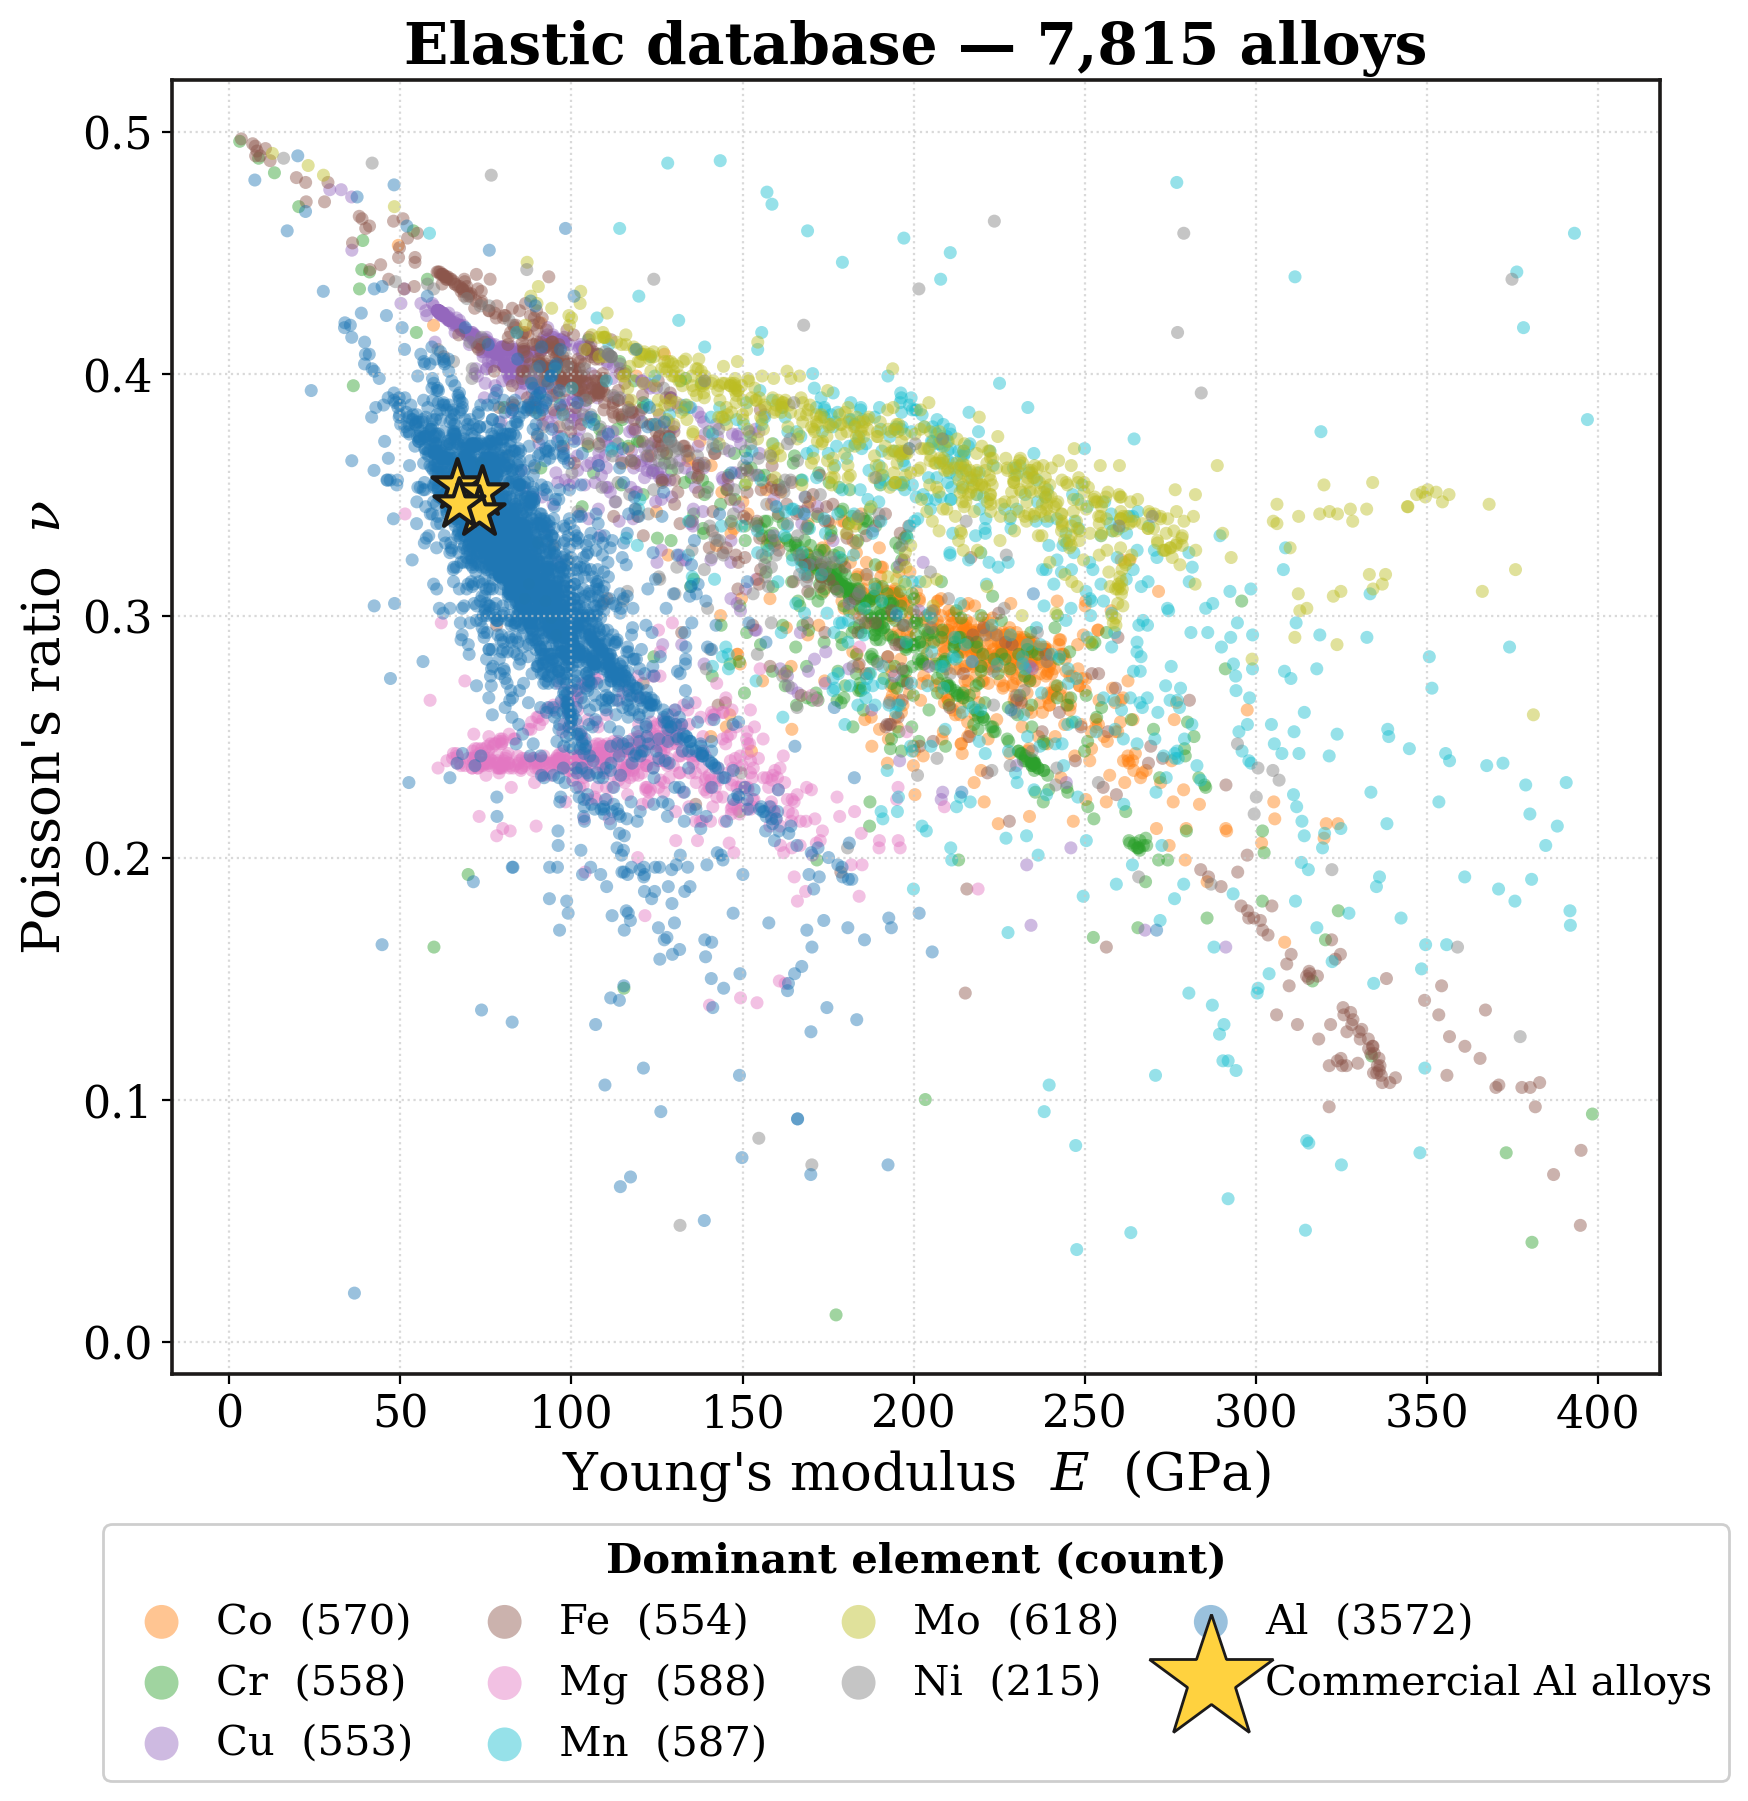
\includegraphics[width=0.96\linewidth]{figures/E_nu_scatter.png}
\figcap{$E$--$\nu$ distribution coloured by dominant element
($N=7\,815$). Named commercial alloys are highlighted.}
\end{minipage}\end{center}

% ------------------------------------------------------------ sec 4
\sect{DFT references \& MEAM initialisation}
Plane-wave PBE--GGA calculations in Quantum Espresso [4] provide each
element's lattice constant $a_0$, cohesive energy $E_{\mathrm{coh}}$
and bulk modulus $B$ from an equation-of-state fit. These pin the
universal binding (Rose) curve [5] and fix the MEAM decay exponent
\[
  \alpha = \sqrt{\,9B\Omega / E_{\mathrm{coh}}\,},
  \qquad \Omega \text{ the atomic volume},
\]
ranging from $\alpha\approx4.5$ (Al, Si) to $10.9$ (Zn) across the
twelve elements (FCC/BCC/HCP/diamond). Sixty-six binary formation
energies seed the sign of each cross-term.

\begin{center}\begin{minipage}{\linewidth}\centering

\includegraphics[width=0.84\linewidth]{figures/formation_energy_heatmap.png}
\figcap{Binary formation energies $E_{\mathrm{form}}(i,j)$ (eV/atom)
from DFT; negative values indicate exothermic mixing.}
\end{minipage}\end{center}

% ------------------------------------------------------------ sec 5
\sect{Composition surrogate (stage 5a)}
A fully connected $12\to32\to20\to2$ network (ReLU) predicts
$(C_{11},C_{12})$ under a Huber loss; $E$ and $\nu$ are then recovered
analytically, since direct $\nu$ regression is ill-conditioned. A deep
ensemble of five seeds provides epistemic uncertainty.

\begin{center}\begin{minipage}{\linewidth}\centering
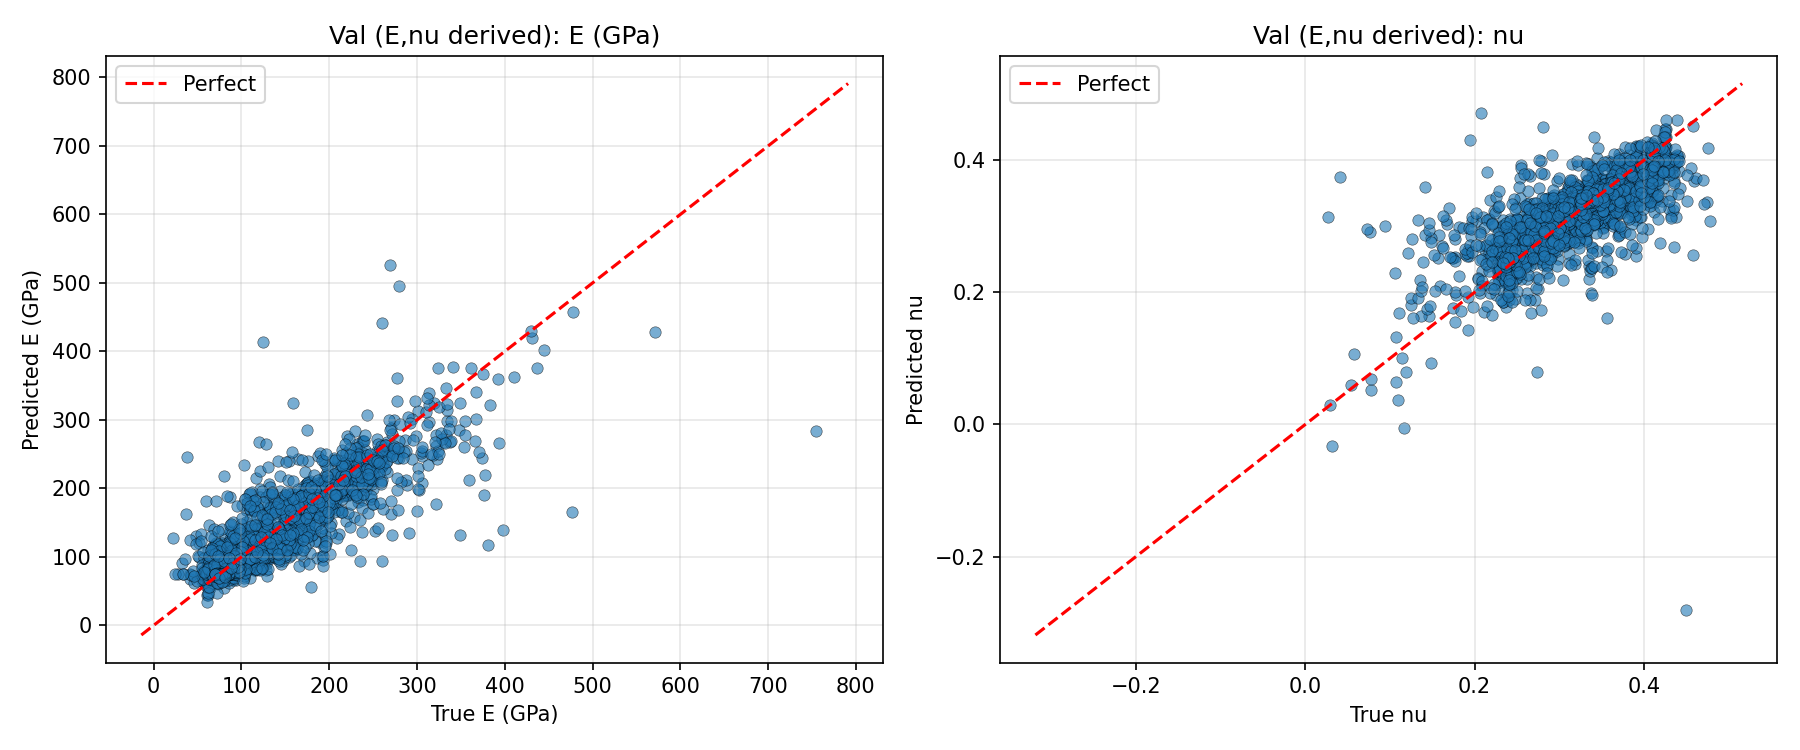
\includegraphics[width=0.88\linewidth]{figures/parity_validation.png}
\figcap{Parity between predicted and MD-computed moduli on the held-out
validation set (30\,\% of the corpus).}
\end{minipage}\end{center}

\begin{keyresult}
$R^{2}_{E}=0.77$, $R^{2}_{\nu}=0.52$ on validation. For Al\,7075 the
surrogate predicts $E=75.5$\,GPa, $\nu=0.334$, against published
$71$--$72$\,GPa and $\nu\approx0.33$ --- within ${\sim}5\%$.
\end{keyresult}

% ------------------------------------------------------------ sec 6
\sect{NN-driven MEAM optimisation (stage 5b)}
A second network learns the map (MEAM parameters) $\to (C_{11},C_{12})$.
It is fitted with Adam [6] on a Huber loss (which decays
$1.0\to0.16$ in training); gradient descent through the \emph{frozen}
surrogate then locates the parameters that reproduce a target
$(C_{11},C_{12})$. Each optimum is re-evaluated in LAMMPS and appended
to the training set, closing the active-learning loop.

\begin{center}\begin{minipage}{\linewidth}\centering
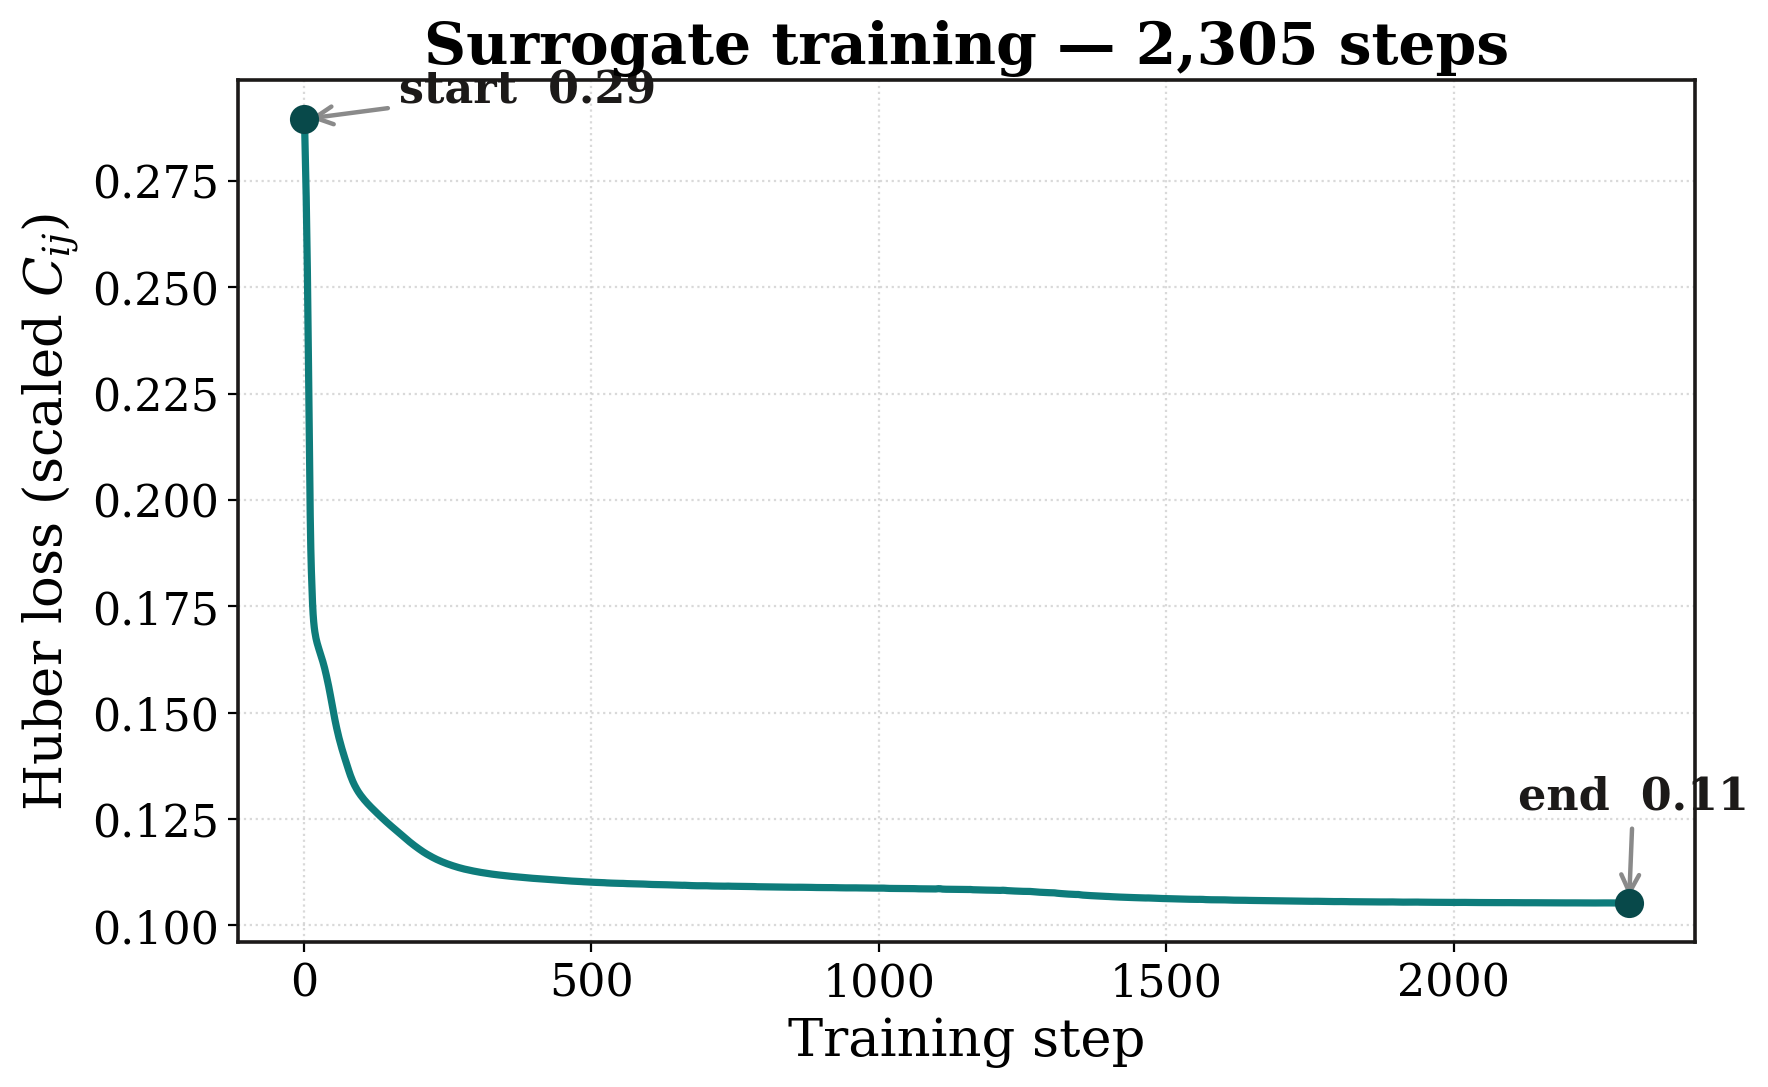
\includegraphics[width=0.84\linewidth]{figures/nnip_training_loss.png}
\figcap{Surrogate training: Huber loss versus epoch for the
parameter-to-$C_{ij}$ network.}
\end{minipage}\end{center}

\begin{center}\begin{minipage}{\linewidth}\centering
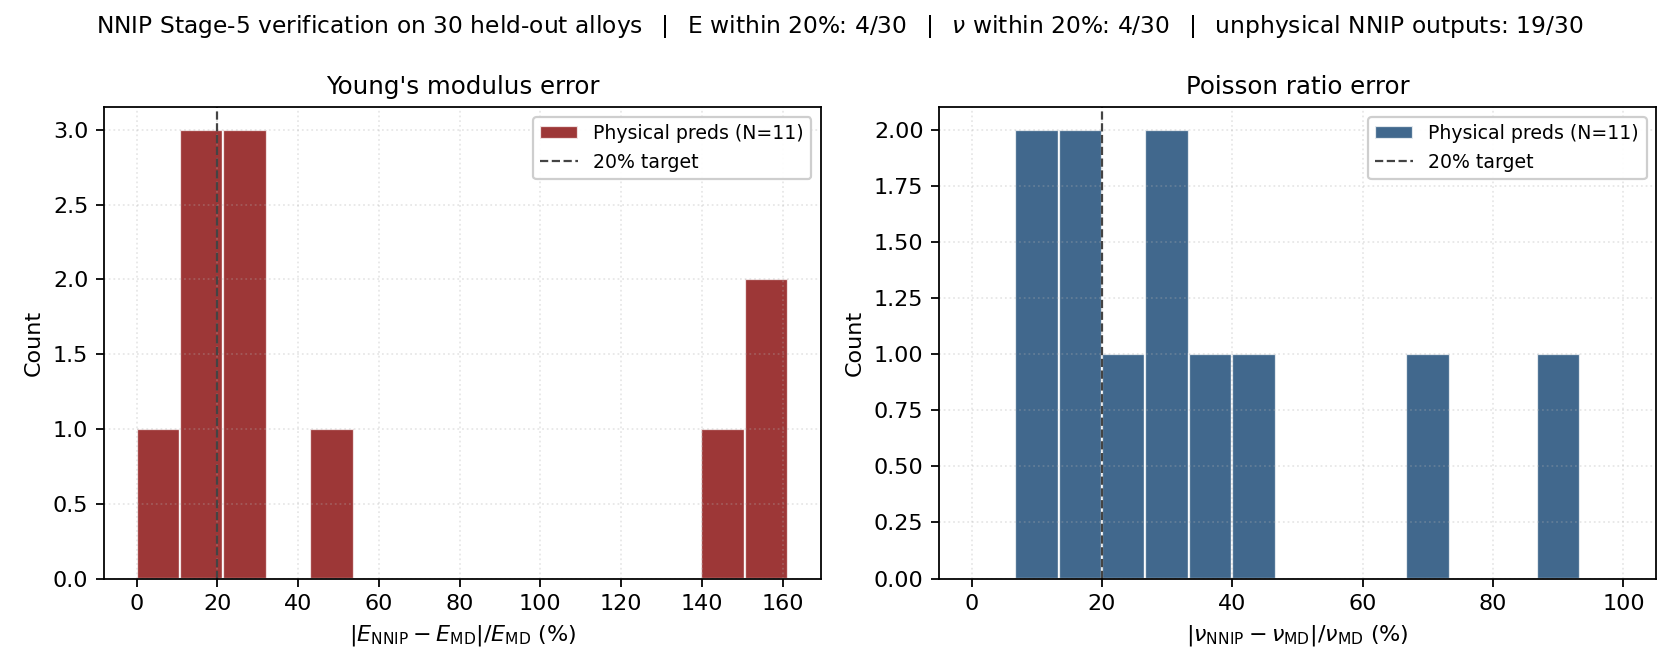
\includegraphics[width=0.94\linewidth]{figures/nnip_verification_errors.png}
\figcap{Verification of the optimized potential against the MD
reference on unseen alloys.}
\end{minipage}\end{center}

\begin{keyresult}
\textbf{Proof of concept.} Of 30 unseen alloys, 11 remained physically
stable under the optimized potential and 4 matched the MD reference
within ${\sim}20\%$. Accuracy grows with more data and longer training.
\end{keyresult}

% ------------------------------------------------------------ sec 7
\sect{Validation against published data}
\begin{center}
\begin{tabular}{lccccc}
\toprule
 & & \multicolumn{2}{c}{$E$ MAPE (\%)} & \multicolumn{2}{c}{$\nu$ MAPE (\%)} \\
\cmidrule(lr){3-4}\cmidrule(lr){5-6}
Family & $N$ & ML & MEAM & ML & MEAM \\
\midrule
Aluminium        & 33 & \textbf{2.3} & 7.4   & 4.0  & 4.5  \\
Titanium         & 6  & 11.6         & 140.0 & 13.2 & 14.6 \\
Stainless        & 3  & 69.6         & 324.1 & 75.5 & 47.3 \\
\midrule
\textbf{Overall} & 43 & \textbf{10.8} & 42.2 & \textbf{7.2} & 7.1 \\
\bottomrule
\end{tabular}
\end{center}
\tabcap{Mean absolute percentage error of the composition surrogate
(ML) and the DFT-initialised potential (MEAM) against published elastic
data, by alloy family.}

Accuracy is strongest where the training corpus is densest
(aluminium); sparse families inherit the corpus bias --- a data
limitation rather than a methodological one.

% ------------------------------------------------------------ sec 8
\sect{Conclusions \& outlook}
\begin{itemize}\setlength\itemsep{0.2em}
  \item An \textbf{automated, end-to-end 12-element MEAM pipeline}:
        from random compositions to an optimized multi-element
        potential with no hand fitting.
  \item \textbf{Aluminium-alloy elastic prediction} from composition
        alone, within a few percent of published values.
  \item \textbf{DFT-seeded, NN-trained MEAM}: first-principles
        references refit through a neural surrogate.
\end{itemize}
Future work: wider composition and crystal-structure coverage, longer
surrogate training per refit, and denser DFT supercell sampling. The
pipeline already runs end to end; what remains is more data, longer
training, and sharper references.

% ------------------------------------------------------------ refs
\vspace{1.1em}
{\color{hairline}\hrule height 0.6pt}\vspace{0.55em}
{\footnotesize
\textbf{References}\par
\begin{enumerate}\setlength\itemsep{0.1em}
  \item M.~I. Baskes, \emph{Phys. Rev. B} \textbf{46}, 2727 (1992).
  \item B.-J. Lee and M.~I. Baskes, \emph{Phys. Rev. B} \textbf{64},
        184102 (2001).
  \item A.~P. Thompson \emph{et al.}, \emph{Comput. Phys. Commun.}
        \textbf{271}, 108171 (2022).
  \item P.~Giannozzi \emph{et al.}, \emph{J. Phys.: Condens. Matter}
        \textbf{21}, 395502 (2009).
  \item P.~Vinet, J.~H. Rose, J.~Ferrante and J.~R. Smith,
        \emph{J. Phys.: Condens. Matter} \textbf{1}, 1941 (1989).
  \item D.~P. Kingma and J.~Ba, \emph{ICLR} (2015).
\end{enumerate}
\textbf{Acknowledgments.} Supervised by Prof.\ Dr.\ Hande Toffoli,
Department of Physics, METU. Computations: LAMMPS
(\texttt{maxelt}${}=20$ patch), Quantum Espresso 7.5, TensorFlow, ASE,
OVITO.\par}

\end{multicols}

\vspace{0.3em}
\begin{tcolorbox}[enhanced, frame hidden, colback=accent, sharp corners,
  left=0mm, right=0mm, top=2.5mm, bottom=2.5mm, boxsep=0mm]
\centering
{\footnotesize\color{white}\itshape PHYS\,400 Senior Project --- Department of
Physics, Middle East Technical University --- 2026\qquad
\textup{\texttt{github.com/canndurmaz/PHYS400}}}
\end{tcolorbox}

\end{document}
